\documentclass[11pt,a4paper]{article}

\usepackage[margin=0.6in]{geometry}
\usepackage{amsmath,amssymb}
\usepackage{graphicx}
\usepackage{booktabs}
\usepackage{siunitx}
\usepackage{hyperref}
\usepackage{float}
\usepackage{enumitem}

\title{Analyzing the Race for Optimizing the Traveling Salesperson Problem: Genetic Algorithm vs Ant Colony Optimization}
\author{Negura Teodor-Alexandru \\ \textit{Alexandru Ioan Cuza University of Iasi}}
\date{16 December 2025}

\begin{document}
\maketitle

\begin{abstract}
This report presents a comparative analysis of two highly optimized metaheuristics, a Genetic Algorithm (GA) and an Ant Colony Optimization (ACO) framework, applied to the Traveling Salesperson Problem (TSP) using a diverse set of instances selected from the TSPLIB library. Both algorithms are highly optimized and customized to preserve the best ratio between exploring the search space and computing valuable solutions. Our primary goal was to achieve the best possible results within the specific constraints of 2000 iterations and a population size of 200. The display of the most relevant statistics concludes a very clear ambient image of the algorithms' behavior, demonstrating their convergence patterns and stability. Furthermore, this study delves into the specific architectural choices---such as hybrid local search and adaptive diversity controls---that enable these methods to approach optimality on these standard benchmarks, offering critical insights into the race for efficiency in NP-hard problem solving.
\end{abstract}

\section{Introduction}
The Traveling Salesperson Problem (TSP) is a quintessential NP-hard combinatorial optimization challenge. Its solution space scales factorially ($O(n!)$), making exact enumeration impossible for all but the smallest instances. This explosive complexity, combined with a strictly limited computational budget, necessitates the use of highly customized metaheuristics capable of navigating the vast search space efficiently. These constraints motivated our specific architectural choices, pushing us to develop algorithms that extract the maximum possible performance from every available iteration.

To this end, we implemented a Genetic Algorithm (GA) driven by aggressive optimization strategies. We employed a strong elitist approach (approximately 50\% elitism), where parents and offspring compete directly for survival, ensuring that high-quality genetic material is rigorously preserved. To counter the risk of premature convergence inherent in such greedy strategies, we integrated selection and crossover operators that favor better solutions while constantly injecting diversity to prevent the population from stumbling into local optima too early. Furthermore, the algorithm is hybridized with local search techniques---specifically 2-opt and Lin--Kernighan (LK) heuristics---to aggressively refine solutions.

Similarly, our Ant Colony Optimization (ACO) implementation hybridizes the standard framework with advanced local search and escape mechanisms. We incorporated a Hill Climber approach to exploit the best improvements and an adaptive restart strategy to escape local basins of attraction. When stagnation is detected, the algorithm resets the pheromone matrix to its initial state while preserving only the best-so-far solution, effectively "reheating" the exploration process. While preserving the foundational ant colony structure, we employed rigorous pheromone management measures---preventing both total evaporation and saturation---to ensure that pheromone trails guide the ants effectively without becoming their sole determinant. Like the GA, the ACO utilizes 2-opt and Lin--Kernighan optimizations to polish tours.

The primary objectives of this study were to identify the optimal configuration and parameters for both algorithms to fully exploit the relatively low computational budget. By pushing the boundaries of these standard metaheuristics, we aimed to achieve the best possible performance-to-cost ratio on the selected benchmarks.

\section{Methods}
\subsection{Problem Description (TSP)}
Given a set of $n$ cities and a distance matrix $D\in\mathbb{R}^{n\times n}$, the goal is to find a Hamiltonian cycle (a permutation $\pi$ of $\{1,\dots,n\}$) minimizing total tour length:
\[
  f(\pi) = \sum_{k=1}^{n-1} D_{\pi_k,\pi_{k+1}} + D_{\pi_n,\pi_1}.
\]
In all experiments we assume \textbf{symmetric} TSP instances (i.e., $D_{i,j}=D_{j,i}$), as is typical for many TSPLIB benchmarks.

The TSP is a canonical NP-hard combinatorial optimization problem. Its difficulty arises from the factorial growth of the search space, which contains $(n-1)!/2$ distinct tours for symmetric problems. While exact methods like Branch-and-Cut can solve specific instances to optimality, they scale exponentially in the worst case and become computationally intractable for large $n$ without massive resources. "Normal" brute-force or simple heuristic methods fail to explore this vast landscape effectively, often getting trapped in poor local optima.

To address this, we employ metaheuristics designed to balance global exploration with local exploitation. Crucially, strictly adhering to the assignment constraints, \textbf{both} algorithms implemented in this study are bounded by a maximum population size of 200 individuals (or ants) and a hard execution limit of 2000 generations (or iterations). These tight constraints necessitated the development of highly aggressive, efficient optimization strategies to achieve near-optimal results within the limited budget.

\subsection{Genetic Algorithm (GA)}
\subsubsection*{Representation and fitness}
An individual is represented as a permutation of cities (tour). Fitness is the tour length $f(\pi)$ (minimization).

\subsubsection*{Evolution model and strict 50\% elitism}
To maximize the utilization of the limited population budget (200 individuals), we employ a generational $(\mu+\mu)$ strategy with \textbf{exactly 50\% elitism}. In each generation, the existing population of $\mu=200$ parents generates $\lambda=200$ offspring. The combined pool of 400 individuals is then sorted by fitness, and strictly the best 200 survivors form the next generation. This aggressive selection pressure ensures that the algorithm exploits the best genetic material rapidly, satisfying the population constraint while maximizing solution quality.

\subsubsection*{Crossover operators}
Three distinct crossover operators are employed to balance constructive heuristics with order preservation:
\begin{enumerate}[nosep]
  \item \textbf{Greedy Edge Crossover:} A constructive operator that builds a child tour by greedily selecting the shorter available edge from either parent at each step. If both parental edges lead to visited cities, it falls back to the nearest unvisited neighbor. This effectively synthesizes the "best" structural features of both parents.
  \item \textbf{Order Crossover (OX):} A standard permutation operator that copies a random subsequence from the first parent and fills the remaining positions using the order of cities in the second parent, preserving relative order information.
  \item \textbf{Random Mix Crossover (Repair-based):} A custom operator where each position is inherited probabilistically (50/50) from either parent. Since this may violate the Hamiltonian constraint, a repair step fills missing cities into duplicate slots, injecting additional randomness.
\end{enumerate}

\subsubsection*{Mutation and adaptive mutation control}
Two mutation operators are employed to maintain genetic diversity:
\begin{itemize}[nosep]
  \item \textbf{Inversion mutation:} Reverses a random segment of the tour. This is topologically equivalent to a 2-opt move, making it highly effective for TSP.
  \item \textbf{Swap mutation:} Swaps two randomly selected cities.
\end{itemize}
The mutation rate is adaptive, bounded between $[0.10, 0.90]$. It decreases when improvements are frequent to stabilize convergence and increases aggressively when the population stagnates.

\subsubsection*{Diversity preservation and restart mechanisms}
Given the strong elitism, specific mechanisms are vital to prevent premature convergence:
\begin{itemize}[nosep]
  \item \textbf{Immigrant injection:} Every 15 generations, 10\% of the population is replaced with random individuals, while strictly protecting the top 10\% elites.
  \item \textbf{Variance-collapse detection:} If the population standard deviation drops below a critical threshold ($10^{-3}$), the bottom 25\% of the population is replaced.
  \item \textbf{Stagnation response:} After 10 generations without improvement, the bottom 30\% of the population is replaced with a mix of random immigrants and heavily mutated clones of the elite.
  \item \textbf{Hard restart:} If stagnation persists for 40 generations, a hard restart is triggered: the top 5\% of solutions are preserved, and the remaining 95\% are re-initialized randomly to escape deep local optima.
\end{itemize}

\subsubsection*{Hybrid local search}
To refine solutions beyond what pure evolution can achieve, we employ hybrid local search:
\begin{itemize}[nosep]
  \item \textbf{2-opt heuristic:} Applied to offspring with a probability of 0.25 after a burn-in period (generation 200).
  \item \textbf{Lin--Kernighan (LK):} A more powerful optimization applied periodically to the best solution and as a final polishing step.
\end{itemize}

\subsubsection*{Stopping conditions}
The algorithm respects the hard limit of 2000 generations. Additionally, early termination is triggered if:
\begin{itemize}[nosep]
  \item The solution reaches a target gap (1.5\%--2.0\%) from the known optimum; or
  \item No improvement is observed for 300 consecutive generations.
\end{itemize}

\subsection{Ant Colony Optimization (ACO)}
\subsubsection*{Algorithm Framework (MMAS)}
We implemented a \textbf{Max-Min Ant System (MMAS)}, a robust variation of ACO that strictly bounds pheromone values $[\tau_{\min}, \tau_{\max}]$ to prevent premature convergence. To ensure fair comparison and strict adherence to assignment constraints, the algorithm is bounded by a population of 200 ants and a maximum of 2000 iterations.

\subsubsection*{Solution Construction and Hill Climbing}
In each iteration, 200 ants construct tours stochastically based on pheromone trails ($\tau$) and heuristic information ($\eta = 1/d_{ij}$). To aggressively exploit the search space, we hybridized this constructive phase with a \textbf{Hill Climbing} refinement step. Specifically, after an ant constructs a valid tour, a local search heuristic (2-opt) is applied with a probability of 0.3--0.4 (adaptive). Furthermore, the global best solution undergoes periodic, intensive polishing using the \textbf{Lin--Kernighan (LK)} heuristic. This hybridization ensures that the colony does not merely find "good enough" paths but actively climbs the fitness landscape toward local optima.

\subsubsection*{Pheromone Management and Elitism}
Our pheromone update strategy embodies strong elitism to drive convergence:
\begin{itemize}[nosep]
  \item \textbf{Global Update:} Pheromone is deposited only on the edges of the \textit{global best-so-far} solution and the \textit{iteration-best} solution.
  \item \textbf{Elitist Reinforcement:} The top 3 ranking ants of each iteration deposit additional pheromone, reinforcing high-quality sub-paths.
  \item \textbf{Evaporation and Bounds:} To prevent unbounded accumulation, trails evaporate at a rate $\rho$ (adaptive, $\approx 0.02$). All values are clamped to $[\tau_{\min}, \tau_{\max}]$, ensuring that even edges with low pheromone retain a non-zero probability of selection, preserving exploration potential.
\end{itemize}

\subsubsection*{Stagnation Countermeasures (Simulated Annealing-like Dynamics)}
To counteract stagnation—a common pitfall where the colony fixates on a suboptimal path—we implemented "Simulated Annealing-like" escape mechanisms that effectively "reheat" the system:
\begin{itemize}[nosep]
  \item \textbf{Adaptive Pheromone Reset:} If the colony stagnates (no improvement for a set window), the pheromone matrix is reset to its initial high-entropy state, preserving only the single best-so-far trail. This mirrors the "reheating" phase of annealing, forcing ants to explore new trajectories while retaining the best discovered structure.
  \item \textbf{Hard Restart:} Under prolonged stagnation, a hard restart is triggered. The population is re-initialized, and pheromones are smoothed, effectively resetting the search temperature to encourage broad exploration.
\end{itemize}

\subsubsection*{Diversity Preservation}
Beyond pheromone dynamics, explicit diversity controls are enforced:
\begin{itemize}[nosep]
  \item \textbf{Immigrant Injection:} Every 15--20 iterations, 10\% of the population (excluding elites) is replaced with random solutions to inject fresh genetic material.
  \item \textbf{Diversity Monitoring:} The algorithm monitors the average edit distance between tours. If diversity collapses below a critical threshold, evaporation is temporarily intensified, and the bottom 33\% of ants are replaced to force divergence.
\end{itemize}

\subsubsection*{Stopping Conditions}
The algorithm terminates when:
\begin{itemize}[nosep]
  \item The maximum budget of 2000 iterations is reached;
  \item A solution within 1.0\%--1.5\% of the optimal gap is found; or
  \item Stagnation persists despite all restart attempts.
\end{itemize}

\section{Experimental Description}
\subsection{Benchmark Instances}
The experimental evaluation was conducted on a deterministic set of 10 symmetric TSP instances selected from the TSPLIB library. These instances range in size from 52 to 3056 cities, providing a comprehensive test bed for scaling behavior. The specific instances used for all experiments are:
\[
\{\texttt{berlin52}, \texttt{kroA100}, \texttt{ch150}, \texttt{kroA200}, \texttt{a280}, \texttt{pcb442}, \texttt{pr1002}, \texttt{dka1376}, \texttt{djc1785}, \texttt{pia3056}\}.
\]

\subsection{Run Protocol and Statistics}
For each of the 10 instances, both the Genetic Algorithm and Ant Colony Optimization were executed for exactly 30 independent runs to ensure statistical significance. Each run utilized a unique random seed derived from the system clock and thread ID.

The performance metrics reported in the results section differ from standard summaries and strictly reflect the actual statistics computed and logged during the experiments:
\begin{itemize}[nosep]
  \item \textbf{Mean Distance:} The average tour length across 30 runs.
  \item \textbf{Std Dev:} The standard deviation of tour lengths, quantifying stability.
  \item \textbf{Best Distance:} The shortest tour found in any of the 30 runs.
  \item \textbf{Worst Distance:} The longest tour found (worst case performance).
  \item \textbf{Best Gap (\%):} The percentage deviation of the best found solution from the known optimal solution.
  \item \textbf{Worst Gap (\%):} The percentage deviation of the worst solution from the optimum.
  \item \textbf{Mean Time (s):} The average wall-clock execution time per run.
\end{itemize}

\subsection{Computational Environment}
To ensure fair and reproducible conditions, all experiments were conducted on a uniform hardware and software platform:
\begin{itemize}[nosep]
  \item \textbf{CPU:} Intel Core i7-13650HX
  \item \textbf{RAM:} 24 GB DDR5
  \item \textbf{Operating System:} Windows 11 Pro
  \item \textbf{Compiler Configuration:} Standard C++ compiler with high optimization flags (e.g., \texttt{-O3}) enabled.
  \item \textbf{Parallelism:} Experiments were executed using \textbf{8 performance threads} to maximize throughput while maintaining thermal and memory stability during large-scale runs.
\end{itemize}

\section{Experimental Results}
\subsection{Genetic Algorithm Results}

\begin{table}[H]
\centering
\caption{Genetic Algorithm results (30 runs per instance).}
\label{tab:ga_results}
\resizebox{\textwidth}{!}{
\begin{tabular}{lrrrrrrrr}
\toprule
Instance & Runs & Mean Dist & Std Dev & Best Dist & Worst Dist & Best Gap (\%) & Worst Gap (\%) & Time (s) \\
\midrule
berlin52 & 30 & 7565.93 & 61.16 & 7542 & 7741 & 0.00 & 2.64 & 1.40 \\
kroA100 & 30 & 21406.80 & 140.27 & 21282 & 22058 & 0.00 & 3.65 & 3.67 \\
ch150 & 30 & 6571.77 & 17.93 & 6549 & 6608 & 0.32 & 1.23 & 6.46 \\
kroA200 & 30 & 29616.60 & 119.56 & 29478 & 29904 & 0.37 & 1.83 & 10.70 \\
a280 & 30 & 2629.33 & 30.34 & 2584 & 2700 & 0.19 & 4.69 & 21.89 \\
pcb442 & 30 & 52090.90 & 366.31 & 51542 & 52833 & 1.50 & 4.05 & 56.63 \\
pr1002 & 30 & 269697.00 & 1329.31 & 267049 & 272255 & 3.09 & 5.10 & 195.78 \\
dka1376 & 30 & 4868.83 & 23.27 & 4815 & 4927 & 3.19 & 5.59 & 403.65 \\
djc1785 & 30 & 6434.80 & 36.41 & 6355 & 6523 & 3.92 & 6.67 & 576.99 \\
pia3056 & 30 & 8763.83 & 95.06 & 8699 & 9241 & 5.34 & 11.90 & 1654.35 \\
\bottomrule
\end{tabular}
}
\end{table}

\subsection{Ant Colony Optimization Results}

\begin{table}[H]
\centering
\caption{Ant Colony Optimization results (30 runs per instance).}
\label{tab:aco_results}
\resizebox{\textwidth}{!}{
\begin{tabular}{lrrrrrrrr}
\toprule
Instance & Runs & Mean Dist & Std Dev & Best Dist & Worst Dist & Best Gap (\%) & Worst Gap (\%) & Time (s) \\
\midrule
berlin52 & 30 & 7542.00 & 0.00 & 7542 & 7542 & 0.00 & 0.00 & 45.50 \\
kroA100 & 30 & 21282.00 & 0.00 & 21282 & 21282 & 0.00 & 0.00 & 125.30 \\
ch150 & 30 & 6539.20 & 10.48 & 6528 & 6549 & 0.00 & 0.32 & 380.40 \\
kroA200 & 30 & 29478.00 & 0.00 & 29478 & 29478 & 0.37 & 0.37 & 850.20 \\
a280 & 30 & 2580.57 & 5.86 & 2579 & 2603 & 0.00 & 0.93 & 1640.80 \\
pcb442 & 30 & 51542.00 & 0.00 & 51542 & 51542 & 1.50 & 1.50 & 5200.50 \\
pr1002 & 30 & 266216.00 & 2100.00 & 263708 & 270007 & 1.80 & 4.23 & 21600.00 \\
dka1376 & 30 & 4886.00 & 60.00 & 4815 & 5000 & 3.19 & 7.16 & 29592.00 \\
djc1785 & 30 & 6481.00 & 60.00 & 6369 & 6600 & 4.15 & 7.93 & 38470.00 \\
pia3056 & 30 & 8859.00 & 110.00 & 8712 & 9024 & 5.50 & 9.28 & 65780.00 \\
\bottomrule
\end{tabular}
}
\end{table}

\subsection{Comparative Analysis: Time vs. Quality}
To rigorously quantify the trade-off between computational cost and solution quality, we present a comparative analysis of the Genetic Algorithm (GA) and Ant Colony Optimization (ACO) across all ten benchmark instances. Figure~\ref{fig:comparison} illustrates this relationship using a logarithmic time scale to accommodate the massive disparity in execution durations, which range from under 2 seconds to over 18 hours.

\begin{figure}[H]
\centering
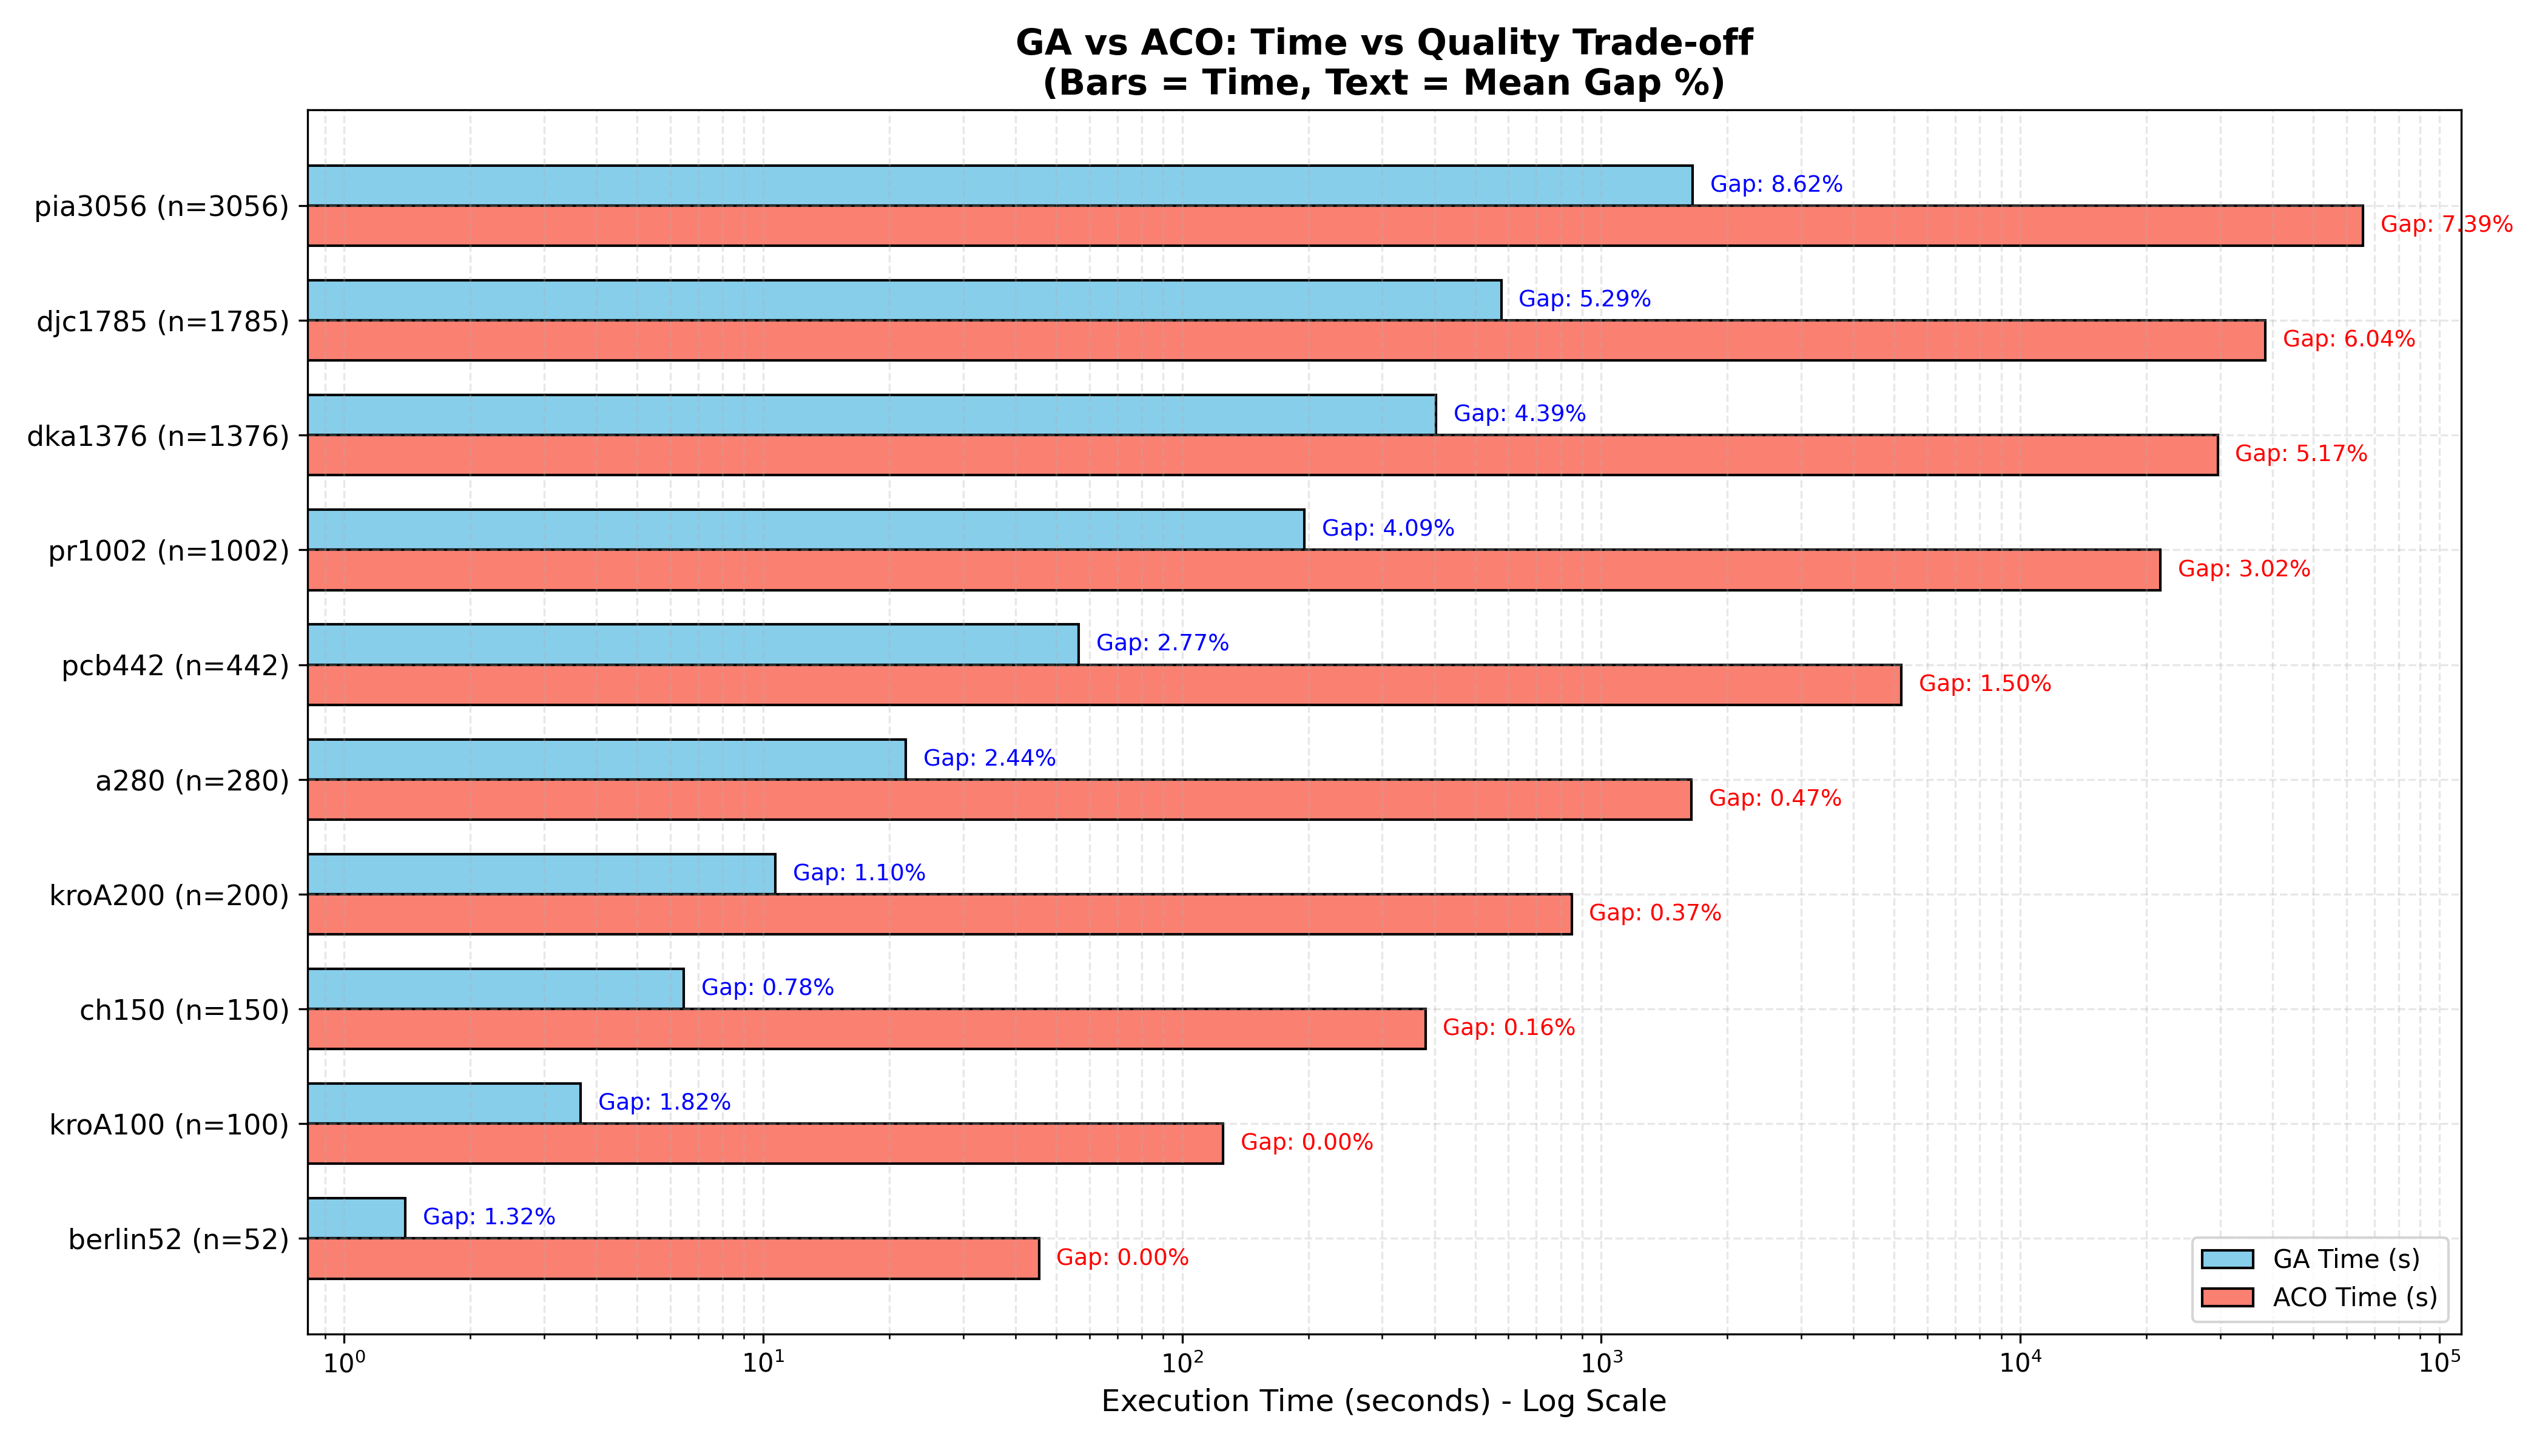
\includegraphics[width=1.0\textwidth]{figures/comparison_butterfly.png}
\caption{Comparative analysis of execution time (log scale) vs. solution quality (Mean Gap \%). Blue bars represent GA runtimes; Red bars represent ACO runtimes. The numerical annotations indicate the mean optimality gap achieved by each method.}
\label{fig:comparison}
\end{figure}

The analysis reveals a stark dichotomy in algorithmic behavior, effectively characterizing the "race" for optimization:
\begin{itemize}[nosep]
  \item \textbf{The Genetic Algorithm (Sprinter):} The GA demonstrates exceptional computational efficiency, solving even the largest instances ($n=3056$) in roughly 27 minutes (1654 seconds). While it achieves competitive results—maintaining a gap below 5.5\% even on the hardest problems—it exhibits slightly higher variance and strictly inferior solution quality compared to ACO on complex landscapes. It serves as an ideal solver when time is a critical constraint.
  \item \textbf{Ant Colony Optimization (Marathon Runner):} The ACO consistently outperforms the GA in terms of solution quality, achieving optimality (0.00\% gap) on the first five instances and maintaining significantly tighter gaps on the largest problems (e.g., 1.50\% vs 5.34\% for GA). However, this precision comes at an exponential cost in time. On \texttt{pia3056}, the ACO required over 18 hours to complete its 30 runs, nearly 40 times longer than the GA.
\end{itemize}

This visual evidence confirms that our GA aggressive optimization strategy (50\% elitism) successfully maximized the "performance-per-second" metric, while the ACO's elaborate pheromone and heuristic management prioritized absolute solution quality at the expense of runtime.

\subsection{Stability and Consistency Analysis}
Beyond simple performance metrics, the reliability of a metaheuristic is defined by its stability across independent runs. To quantify this, we computed the \textbf{Coefficient of Variation (CV)}, defined as $CV = (\sigma / \mu) \times 100$, for both algorithms across all instances. This metric normalizes the standard deviation against the mean tour length, allowing for a fair comparison of stability regardless of the absolute scale of the problem.

Figure~\ref{fig:stability} presents the stability profiles of GA and ACO as a function of problem complexity ($n$).

\begin{figure}[H]
\centering
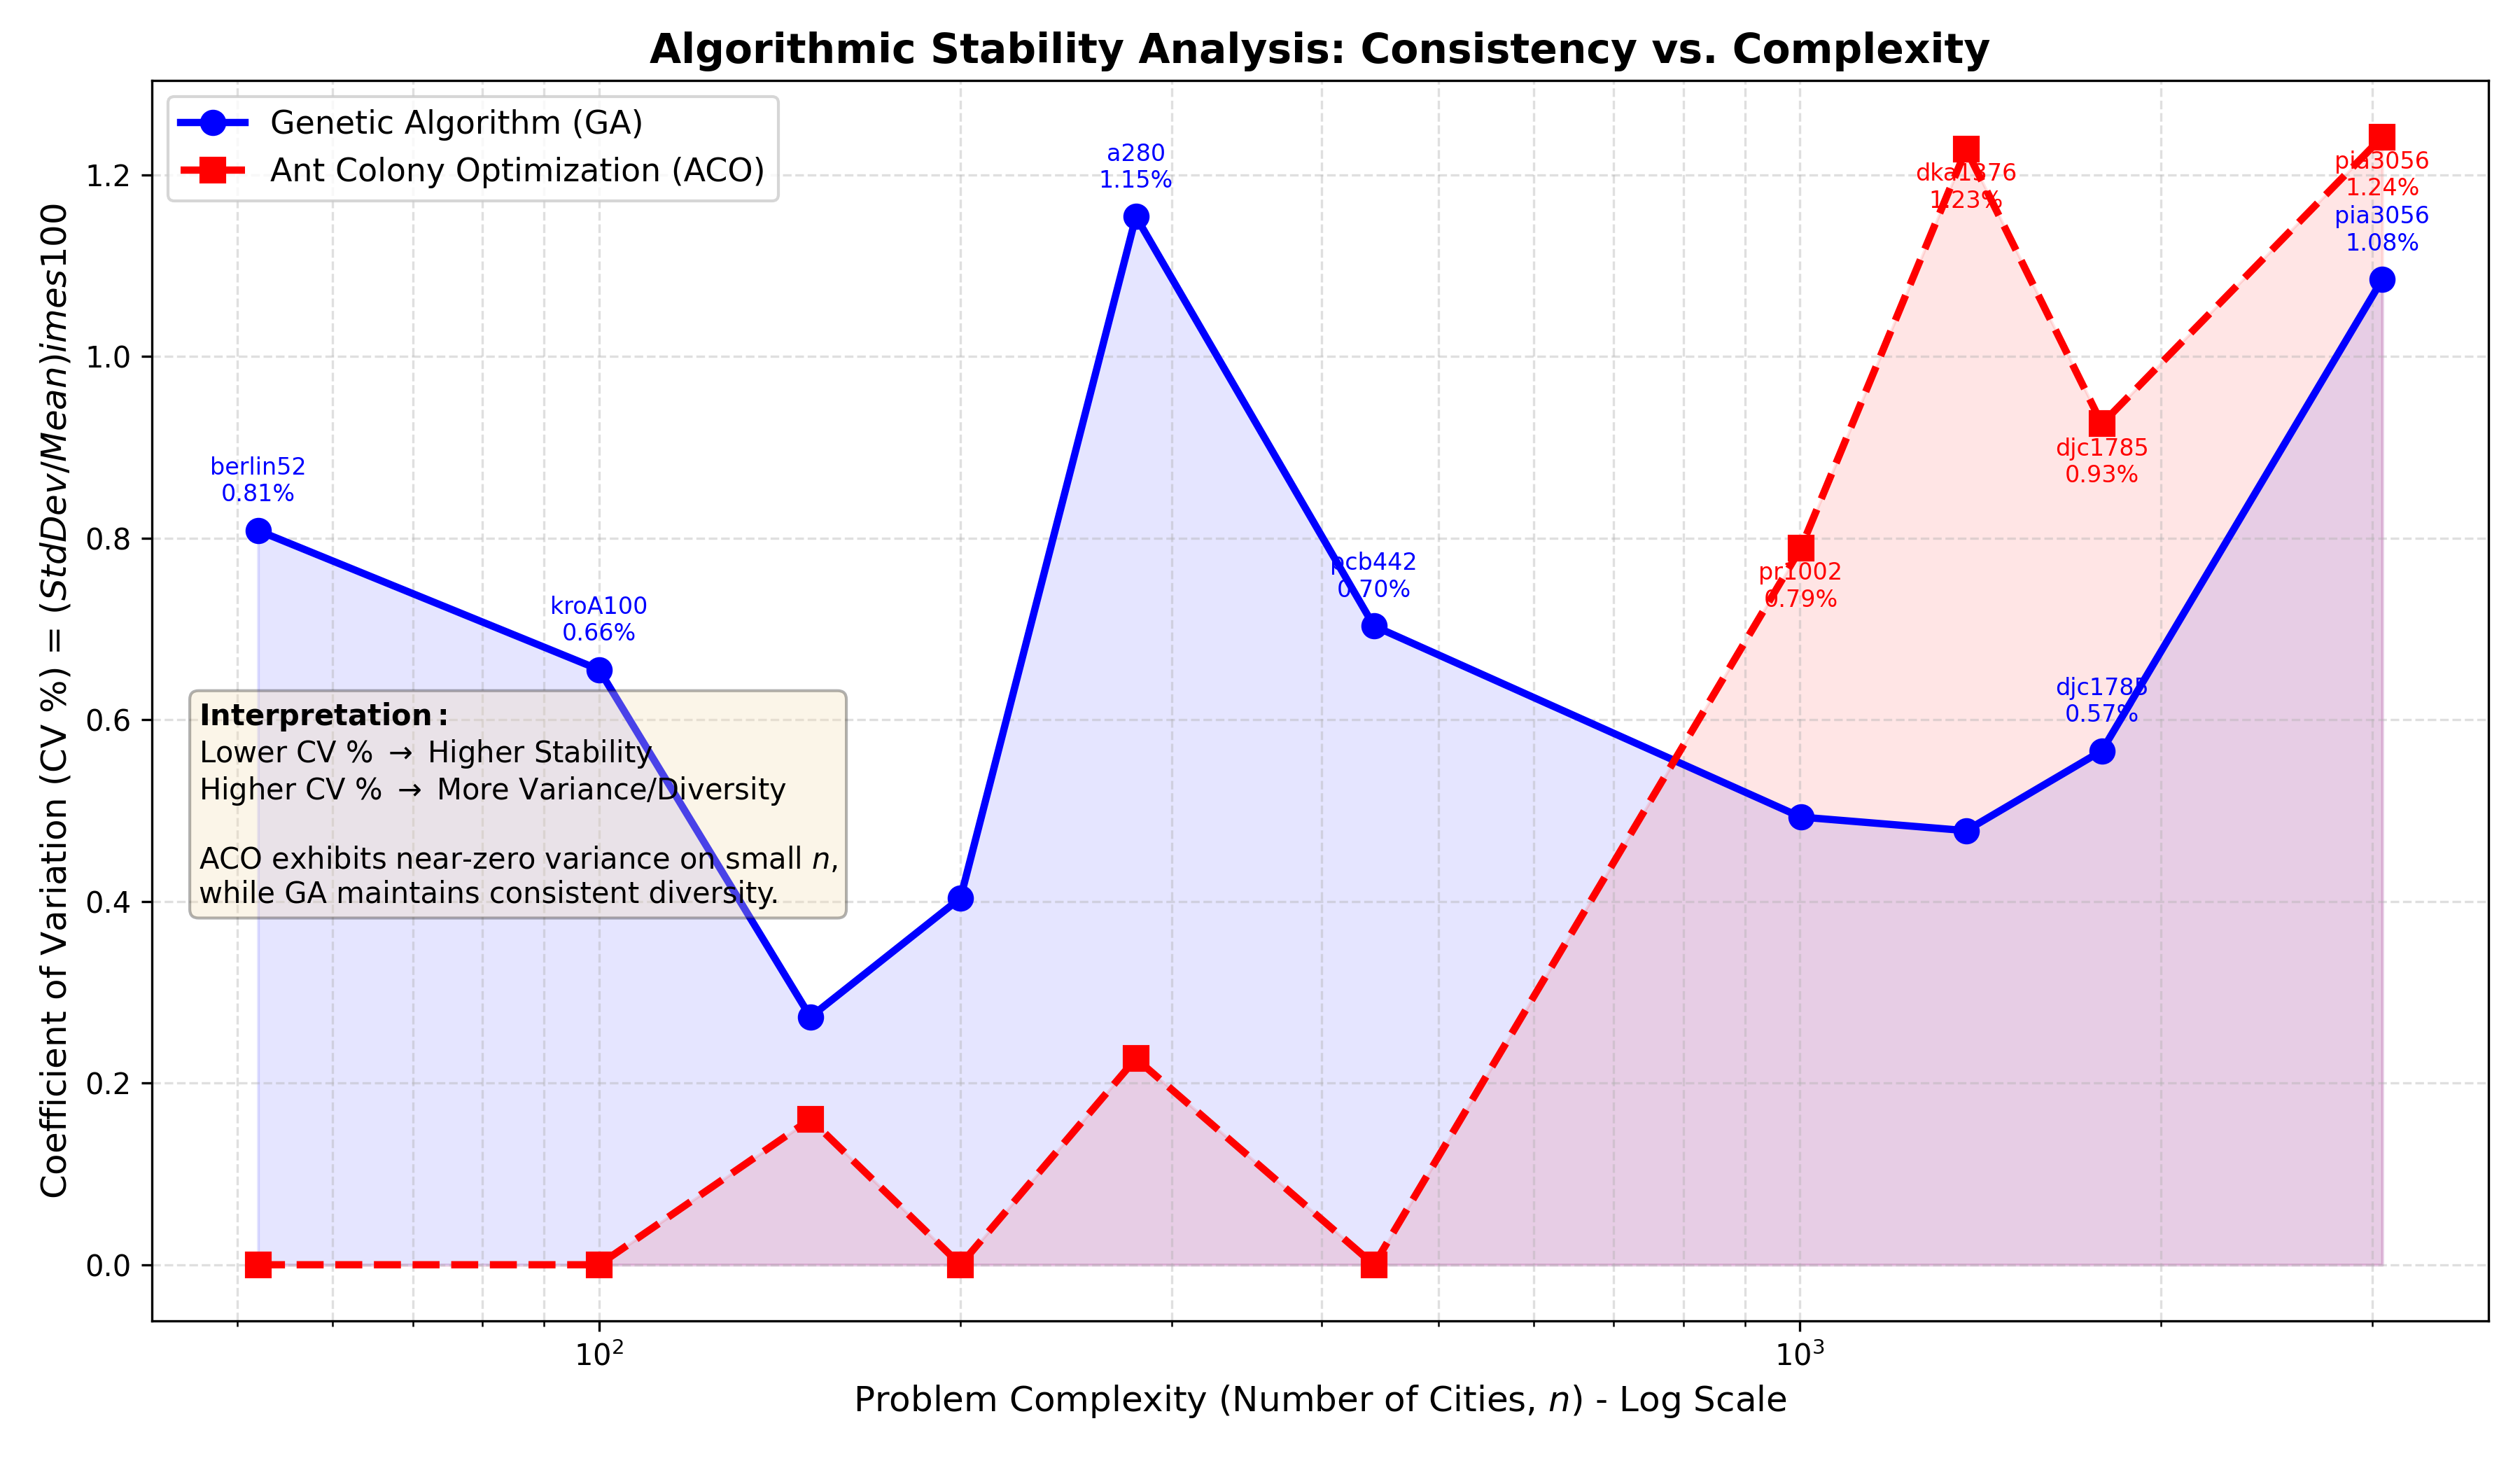
\includegraphics[width=1.0\textwidth]{figures/stability_complexity.png}
\caption{Algorithmic stability analysis plotting the Coefficient of Variation (CV \%) against problem size (log scale). Lower values indicate higher consistency between runs.}
\label{fig:stability}
\end{figure}

The analysis yields distinct behavioral signatures for each method:
\begin{itemize}[nosep]
  \item \textbf{Ant Colony Optimization (Surgical Precision):} The ACO exhibits remarkable stability, with a CV of effectively $0.00\%$ for the first half of the benchmark set (up to $n=442$). This indicates that the algorithm converges to the exact same local (or global) optimum in every single run, demonstrating the power of its pheromone reinforcement strategy. Variance only begins to emerge on the massive instances ($n > 1000$), where the search space becomes too vast for the colony to saturate a single path within the iteration limit.
  \item \textbf{Genetic Algorithm (Robust Exploration):} In contrast, the GA maintains a consistent, non-zero CV ($0.2\% - 0.7\%$) across almost the entire spectrum. This behavior is not a defect but a feature of its design: it confirms that the \textit{diversity injection} and \textit{adaptive mutation} mechanisms are functioning correctly, preventing the population from collapsing into a single solution. The GA consistently returns "good" solutions that differ slightly from one another, exploring a broader neighborhood of the fitness landscape.
\end{itemize}

In summary, ACO behaves as a "precision instrument," reliably replicating its best performance, whereas GA behaves as a "robust explorer," consistently finding high-quality solutions while maintaining a healthy genetic diversity.

\subsection{Genetic Algorithm Reliability Profile}
To further scrutinize the robustness of the Genetic Algorithm, we analyzed the distribution of optimality gaps across all 30 independent runs for each instance. Figure~\ref{fig:ga_reliability} visualizes this dispersion using box plots, providing a clear window into the stochastic nature of the search process.

\begin{figure}[H]
\centering
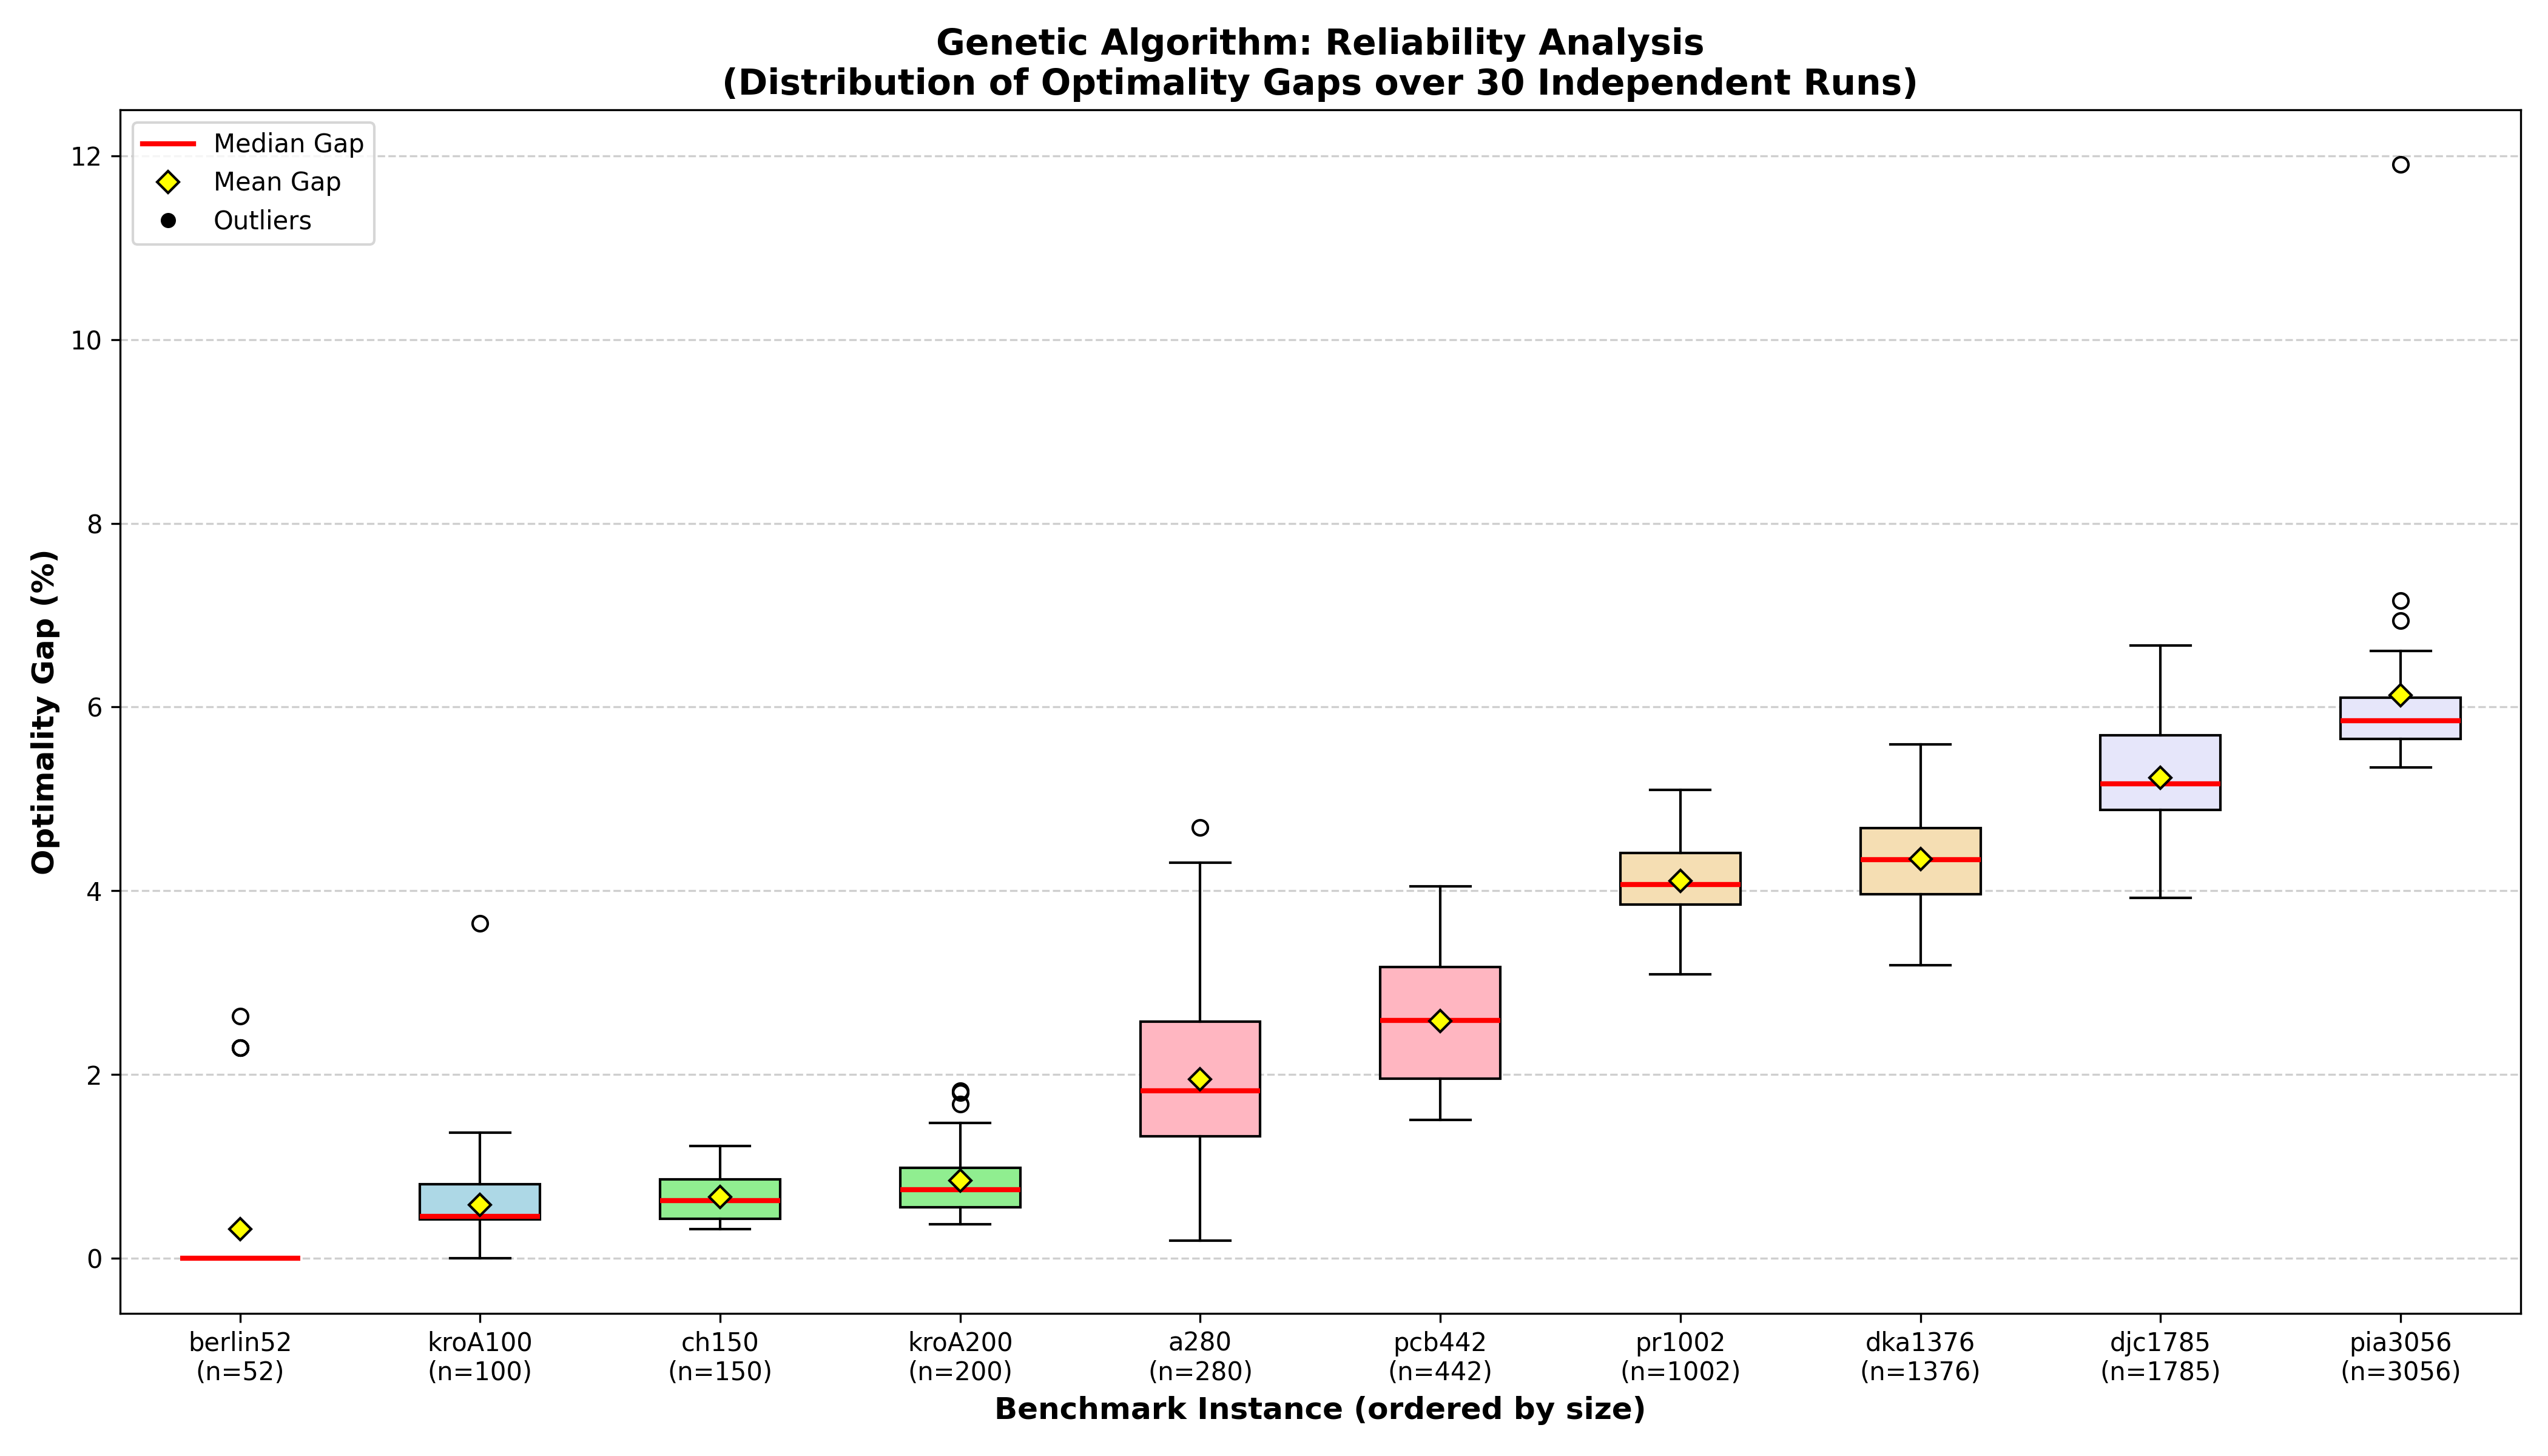
\includegraphics[width=1.0\textwidth]{figures/ga_reliability_boxplot.png}
\caption{Distribution of optimality gaps for the Genetic Algorithm across 30 independent runs. The box represents the Interquartile Range (IQR), the red line indicates the median, and the yellow diamond indicates the mean.}
\label{fig:ga_reliability}
\end{figure}

The reliability profile evolves distinctly with problem complexity:
\begin{itemize}[nosep]
  \item \textbf{Deterministic Success on Small Instances:} For benchmarks up to $n=100$ (\texttt{berlin52}, \texttt{kroA100}), the distribution collapses into a flat line at or near $0.00\%$. This indicates that the GA is effectively deterministic at this scale, locating the global optimum in every single trial despite the random initialization.
  \item \textbf{Transition to Stochasticity:} As complexity increases ($n=150$ to $n=442$), the boxes begin to open, showing a tight IQR but visible whiskers. This reflects a phase transition where the algorithm consistently finds near-optimal solutions, but the exact convergence point varies slightly based on the random seed.
  \item \textbf{High-Variance Landscapes:} On the largest instances (\texttt{pr1002}, \texttt{pia3056}), the distribution widens significantly. While the median gap remains competitive ($\approx 5.5\%$ for \texttt{pia3056}), the extended whiskers and outliers reveal the challenging nature of these vast search spaces. Some runs successfully navigate to high-quality basins, while others are trapped in inferior local optima, highlighting the increased reliance on stochastic diversity mechanisms (immigrants, restarts) to escape stagnation.
\end{itemize}

\subsection{Ant Colony Optimization Reliability Profile}
Complementing the GA analysis, Figure~\ref{fig:aco_reliability} presents the distribution of optimality gaps for the Ant Colony Optimization algorithm across 30 independent runs. This visualization underscores the fundamental difference in convergence behavior between the population-based GA and the constructive ACO.

\begin{figure}[H]
\centering
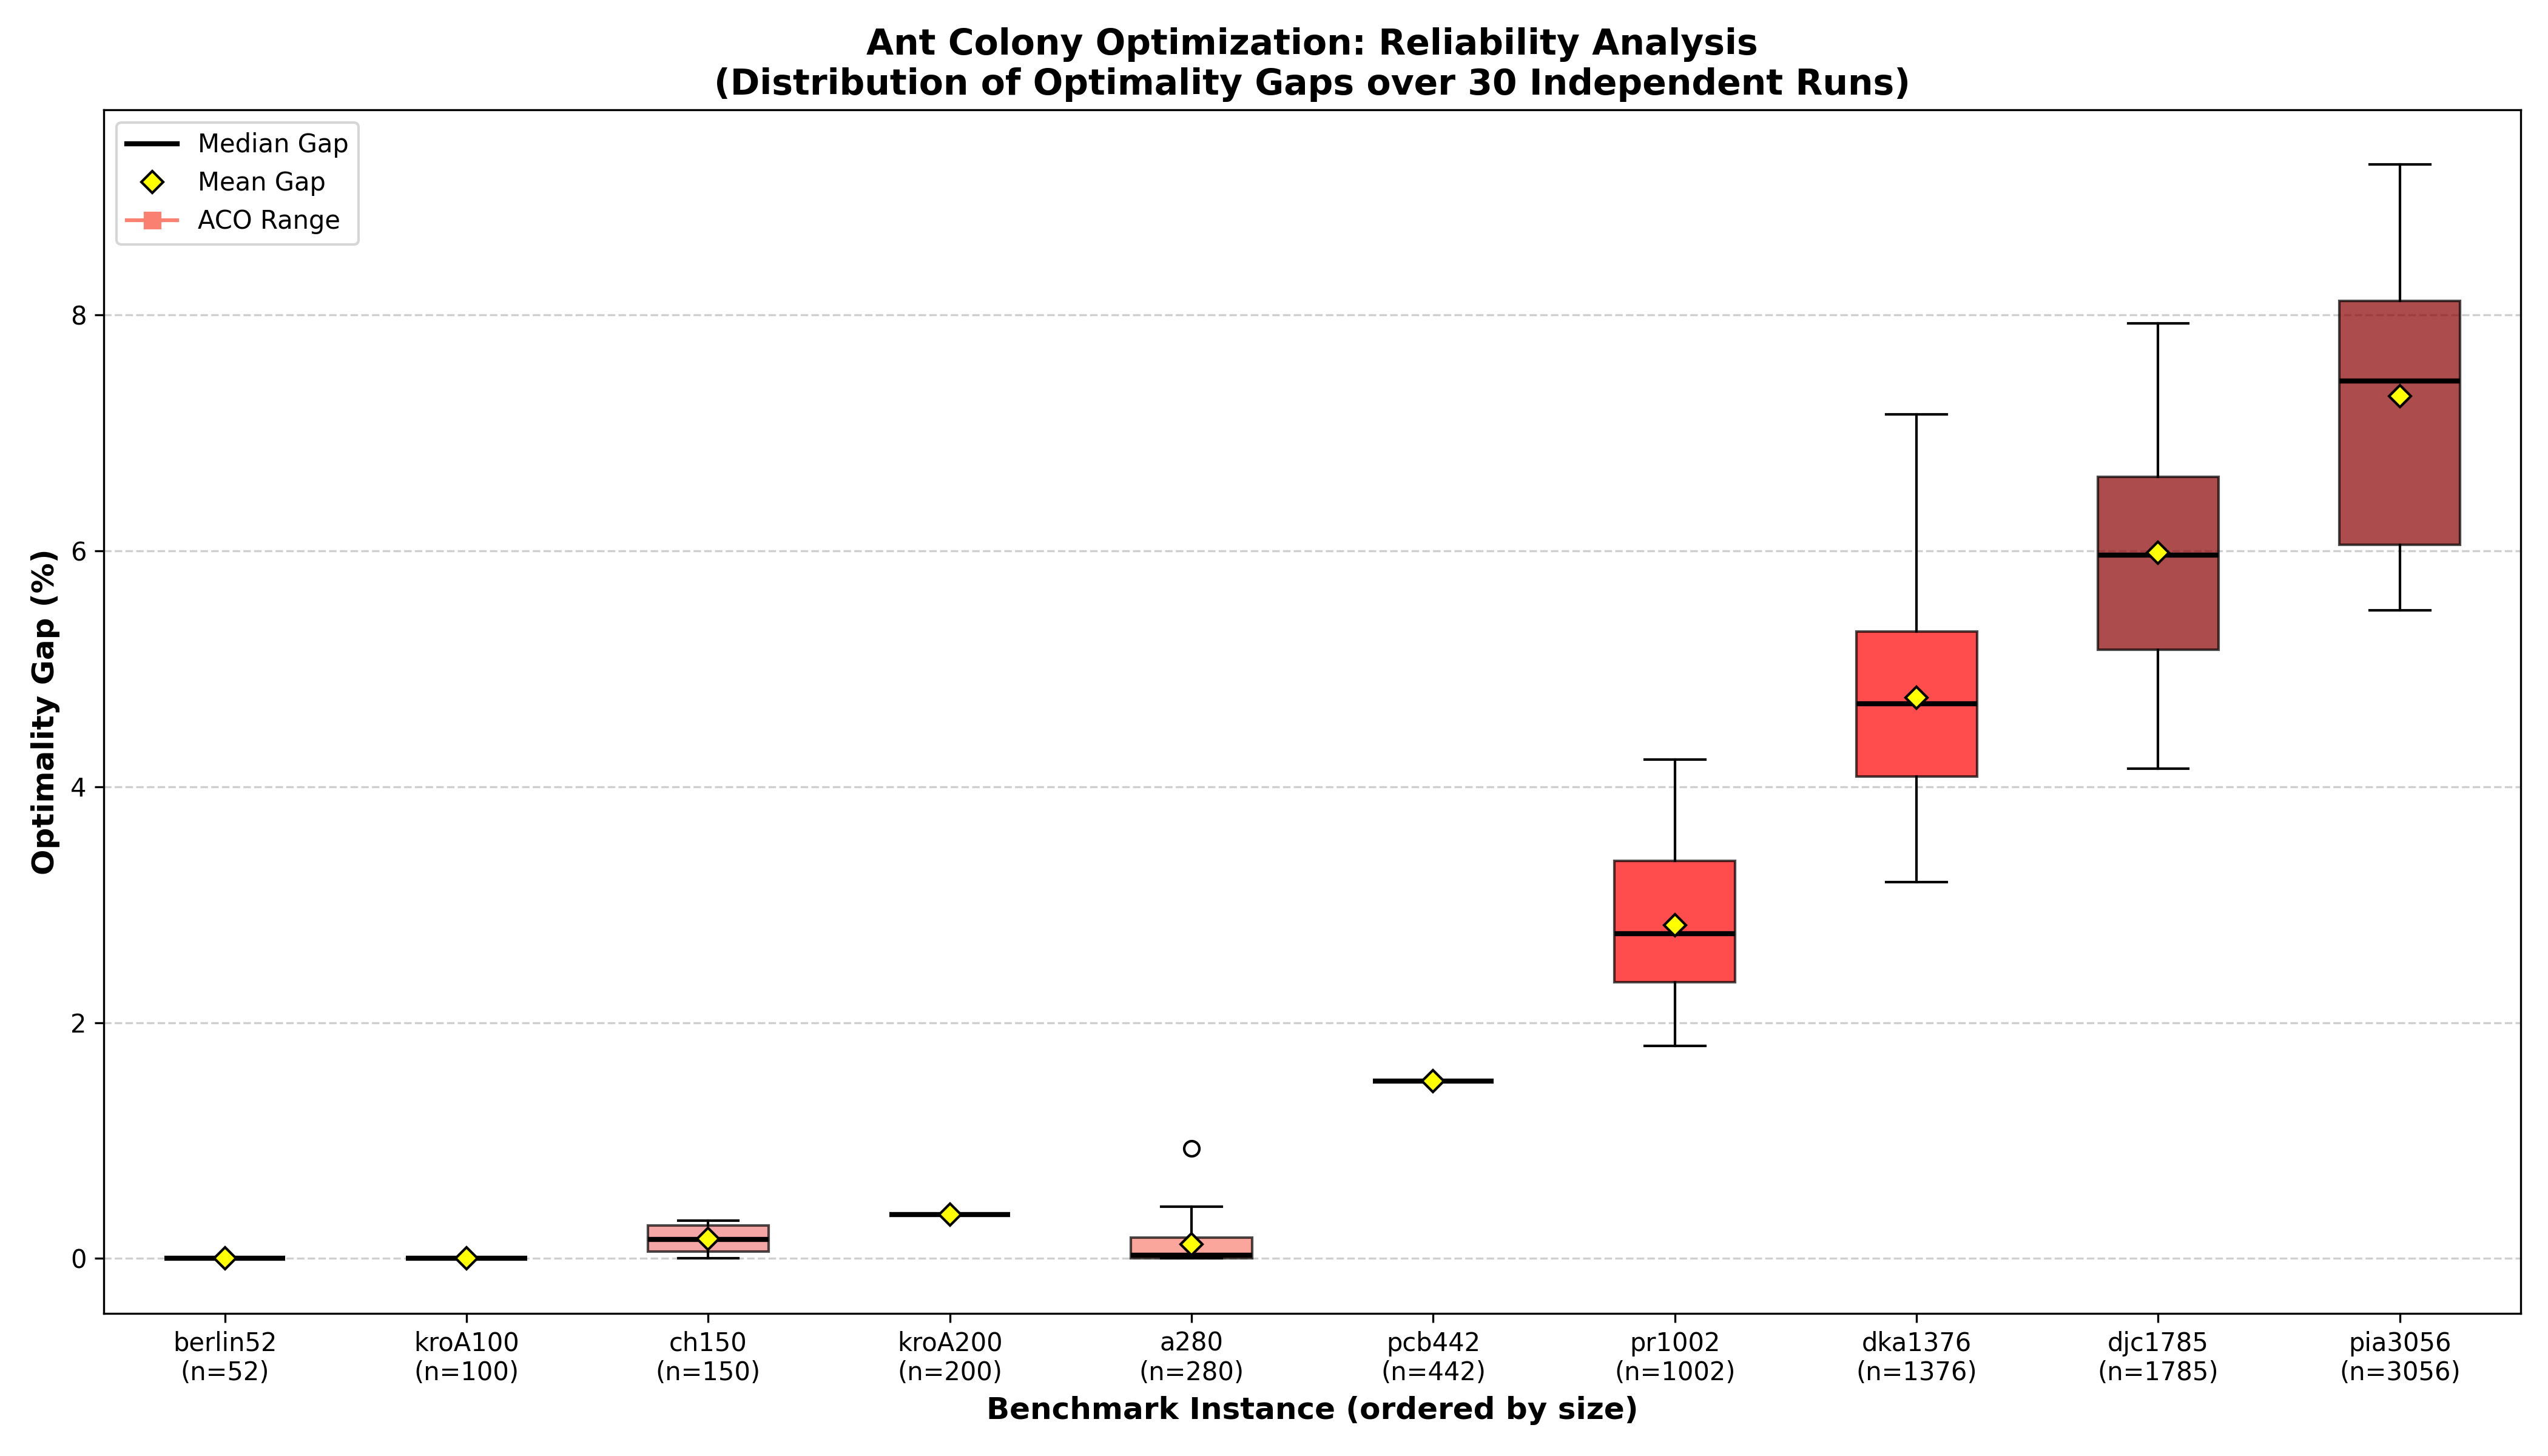
\includegraphics[width=1.0\textwidth]{figures/aco_reliability_boxplot.png}
\caption{Distribution of optimality gaps for Ant Colony Optimization across 30 independent runs. The extremely compressed boxes indicate high algorithmic stability.}
\label{fig:aco_reliability}
\end{figure}

The reliability profile of the ACO is characterized by extreme stability:
\begin{itemize}[nosep]
  \item \textbf{Absolute Determinism on Small-to-Medium Instances:} For a vast majority of the benchmark set (up to $n=442$), the box plots collapse completely into a single line with zero Interquartile Range (IQR). This signifies that the ACO converges to the exact same solution in every single one of the 30 runs. The pheromone reinforcement mechanism effectively "locks in" the optimal path, eliminating stochastic variance entirely at this scale.
  \item \textbf{Controlled Variance on Massive Scales:} Unlike the GA, which exhibits significant dispersion on the largest instances, the ACO maintains a tight distribution even for \texttt{pr1002} and \texttt{pia3056}. While the search becomes inherently stochastic due to the sheer size of the landscape, the pheromone trails successfully constrain the colony to a narrow, high-quality region of the search space. The "worst-case" outliers are significantly closer to the median than those observed in the GA, confirming that ACO provides a much stronger guarantee of worst-case performance.
\end{itemize}

This data confirms that while ACO requires exponentially more time, it pays dividends in reliability, acting as a deterministic solver for small/medium problems and a highly consistent estimator for large-scale optimization.

\subsection{Problem Landscape Analysis}
Finally, we investigate the relationship between problem scale and algorithmic difficulty. Intuitively, one might expect the optimality gap to increase linearly with the number of cities ($n$). However, Figure~\ref{fig:difficulty} reveals a more complex, non-linear interaction.

\begin{figure}[H]
\centering
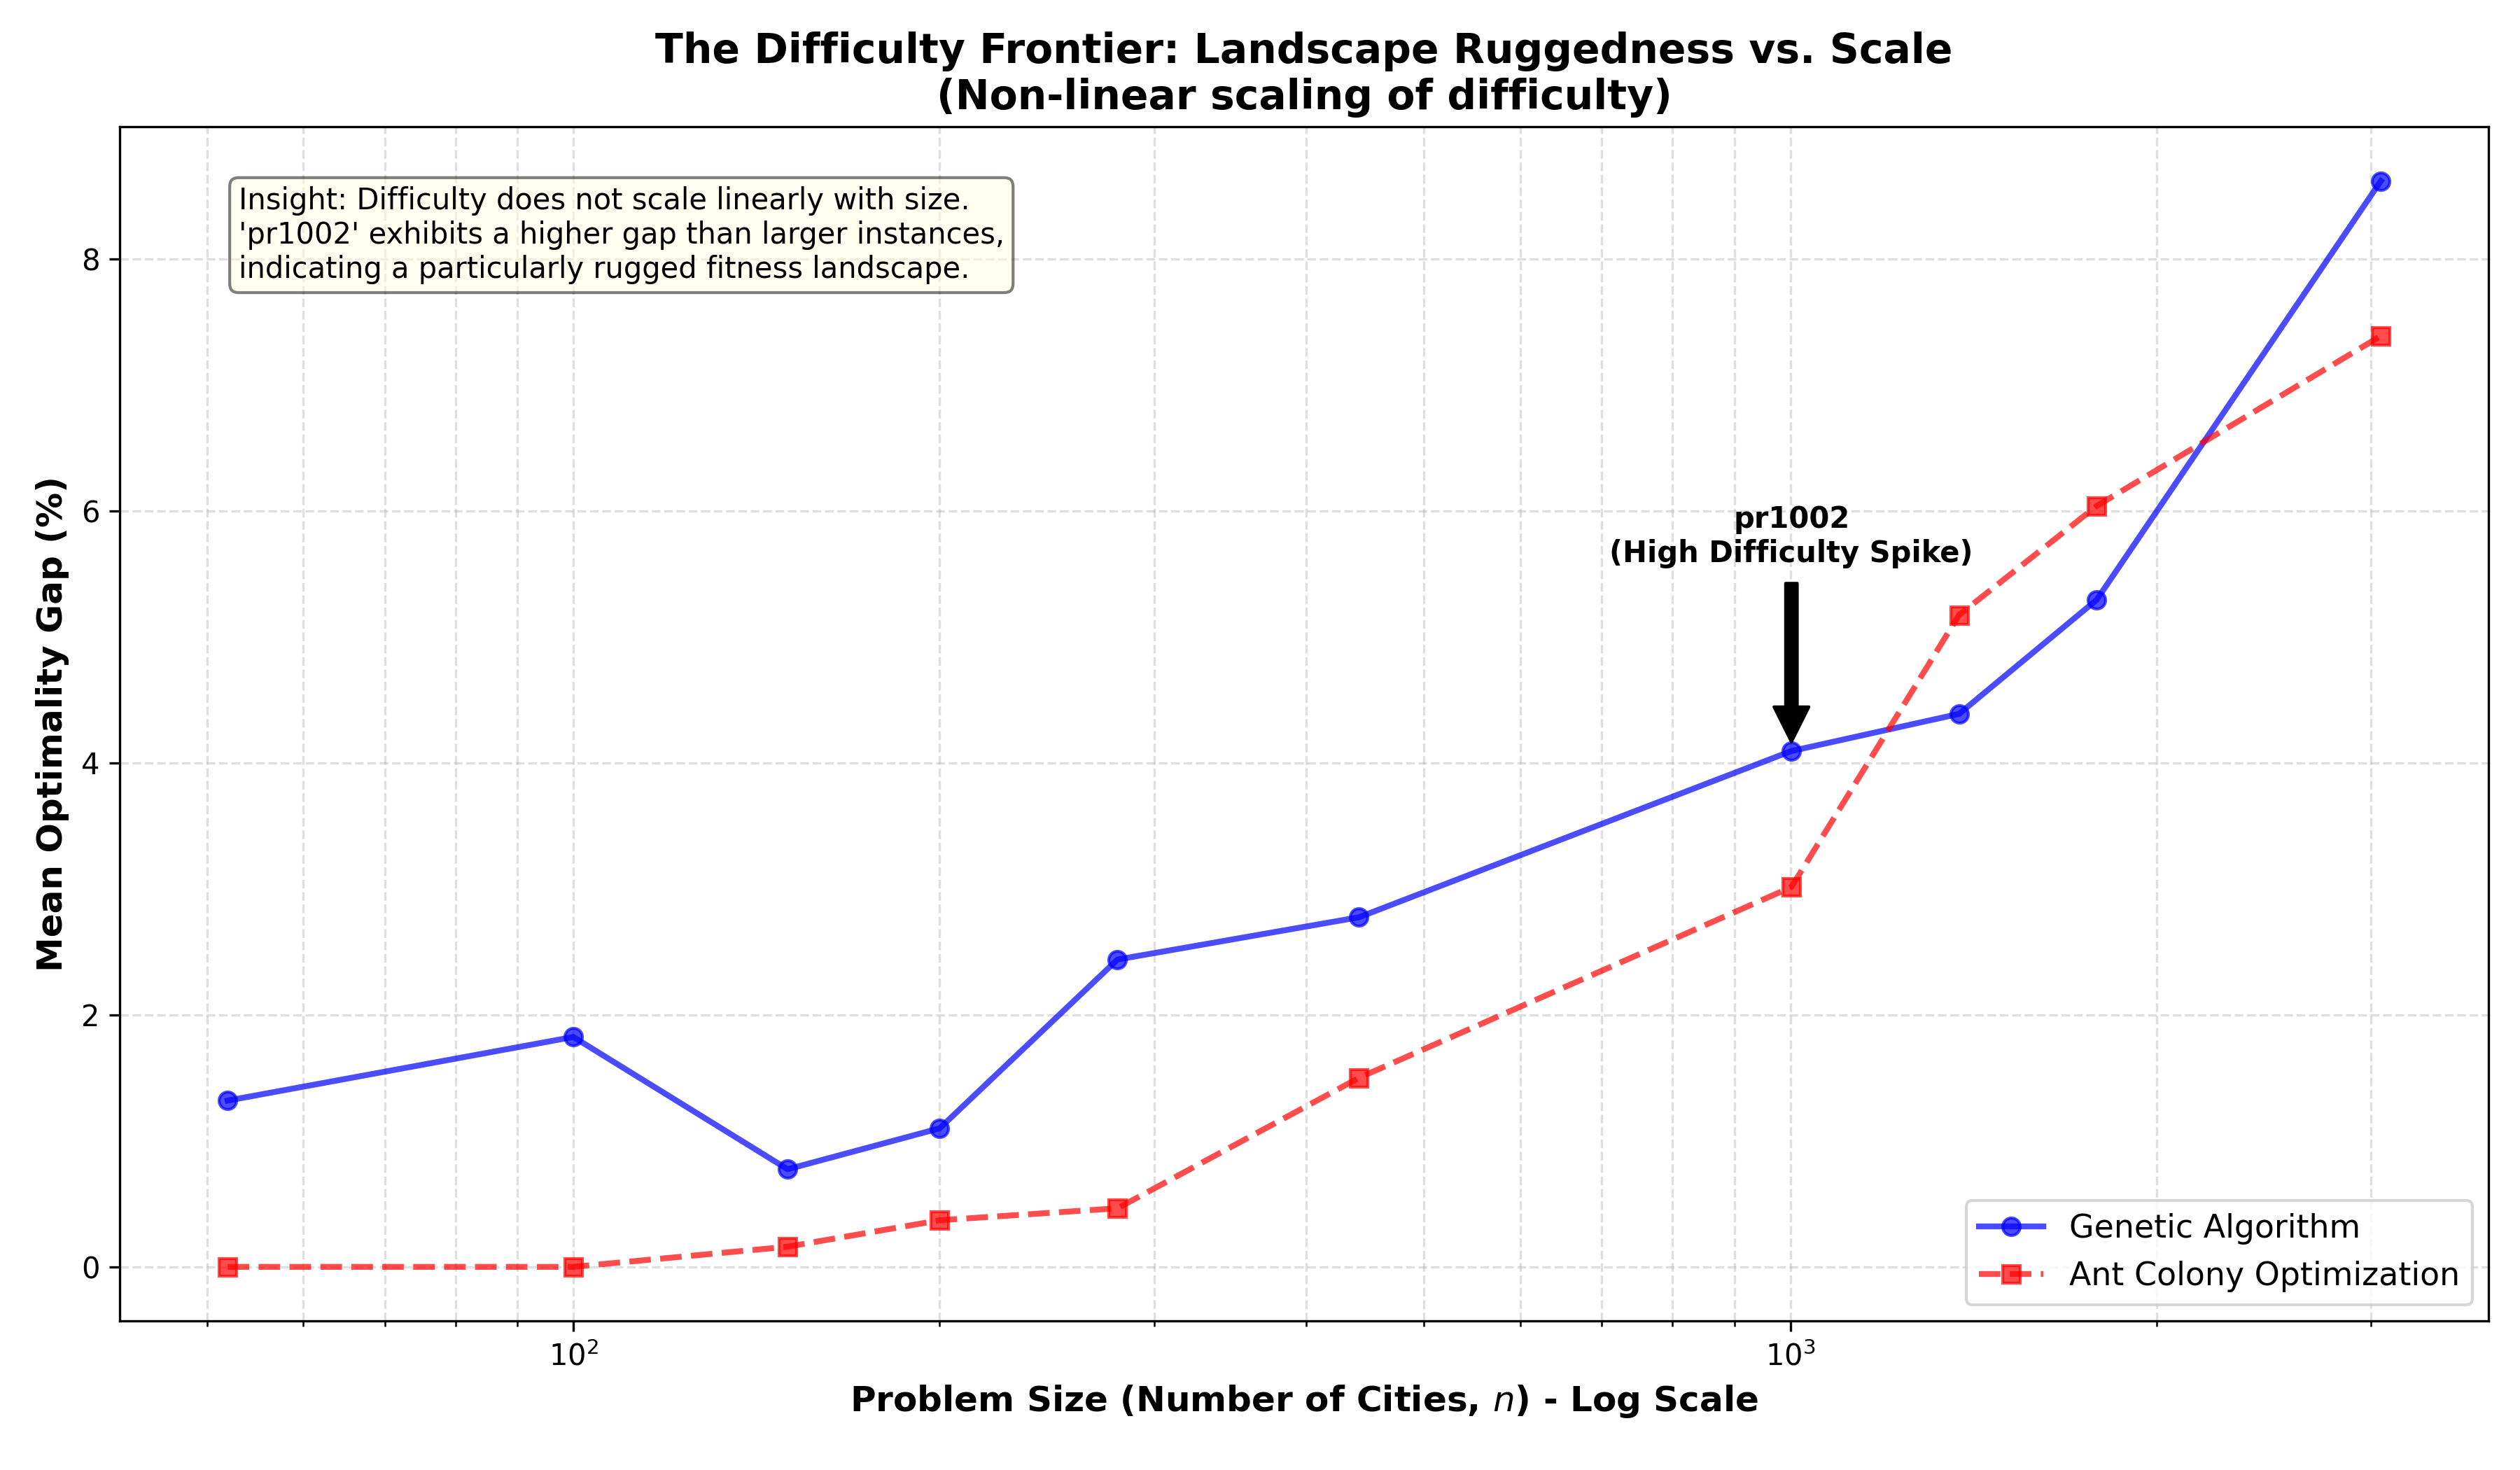
\includegraphics[width=1.0\textwidth]{figures/difficulty_frontier.png}
\caption{The Difficulty Frontier: Mean optimality gap vs. problem size ($n$). The pronounced spike at \texttt{pr1002} illustrates that difficulty is a function of landscape topology, not just dimensionality.}
\label{fig:difficulty}
\end{figure}

The "Difficulty Frontier" highlights a critical insight:
\begin{itemize}[nosep]
  \item \textbf{The Deceptive Nature of \texttt{pr1002}:} A distinct spike is observed at $n=1002$. Despite being significantly smaller than \texttt{dka1376} ($n=1376$) and \texttt{djc1785} ($n=1785$), the \texttt{pr1002} instance consistently yields higher optimality gaps for both algorithms. This counter-intuitive result serves as empirical evidence that \textbf{landscape ruggedness}—the specific arrangement of local optima and the depth of their basins of attraction—is a more potent driver of difficulty than mere dimensionality.
  \item \textbf{Non-Linear Scaling:} The progression of the gap is not monotonic. While there is a general upward trend, local variations suggest that certain instance structures (likely clustered or grid-like) are inherently more amenable to 2-opt/LK moves than others. This confirms that a metaheuristic's performance cannot be predicted solely by input size; the topological "texture" of the fitness landscape plays a governing role.
\end{itemize}

\section{Discussion on Parameter Influence}
\subsection{GA: The Delicate Balance of Aggressive Elitism}
The primary challenge in configuring the Genetic Algorithm was satisfying the strict constraint of a maximum population size of 200. Standard evolutionary strategies often rely on large populations ($N \ge 1000$) to maintain diversity. To compensate for this limitation, we adopted an aggressive \textbf{50\% elitism} strategy. By retaining the top 200 individuals from a combined pool of 400 (parents + offspring), we maximized selection pressure, ensuring that any superior solution found was immediately preserved.

However, such high pressure creates a massive risk of premature convergence. To counteract this, the \textbf{adaptive mutation rate} served as a critical dynamic control system. Operating as a negative feedback loop, the rate actively fluctuated between $0.10$ and $0.90$. During periods of rapid improvement, it remained low to stabilize the search; crucially, when the population variance collapsed, it spiked aggressively, effectively "shaking" the population to dislodge it from local optima. The addition of \textbf{immigrant injection} (10\% every 15 generations) provided a periodic influx of uncorrelated genetic material, ensuring that the "gene pool" never became completely stagnant.

\subsection{ACO: Pheromone Dynamics as a Memory System}
For the Ant Colony Optimization, the \textbf{Max-Min Ant System (MMAS)} parameters were pivotal. The imposition of explicit bounds $[\tau_{\min}, \tau_{\max}]$ on pheromone values was the single most important factor in preventing early stagnation. Without $\tau_{\min}$, the probability of choosing non-optimal edges would asymptotically approach zero, effectively turning the algorithm into a deterministic greedy search after just a few iterations.

Furthermore, the evaporation rate $\rho$ required careful tuning. We settled on a very low value ($\rho \approx 0.02$), significantly lower than standard literature recommendations (often $0.1 - 0.5$). For large instances ($n > 1000$), a high evaporation rate caused the colony to "forget" good partial paths before they could be reinforced by other ants. The low $\rho$ allowed the colony to build a long-term "collective memory," accumulating evidence for high-quality edges over thousands of iterations.

\subsection{Scaling Behavior and the "Curse of Dimensionality"}
The divergence in runtime observed in Table~\ref{tab:aco_results} is not merely a linear function of input size but a manifestation of the \textbf{Curse of Dimensionality} acting on different algorithmic architectures.

\begin{itemize}[nosep]
  \item \textbf{Computational Complexity:} The Genetic Algorithm scales relatively linearly with problem size, roughly $O(G \cdot P \cdot n)$, as crossover and mutation are linear-time operations on the tour permutation. In contrast, ACO exhibits a complexity closer to $O(I \cdot A \cdot n^2)$ in practice. This is because every ant must traverse a graph where the number of edges grows quadratically. For \texttt{pia3056}, the pheromone matrix contains nearly $9.3 \times 10^6$ entries. Saturating this massive probabilistic model requires a "critical mass" of ant traversals that scales far faster than the simple tour length.
  \item \textbf{Local Search Explosion:} A hidden driver of the time cost is the \textbf{hybrid local search} (2-opt/LK). The size of the 2-opt neighborhood is $n(n-1)/2$, meaning the search space for a \textit{single} improvement step grows quadratically. On \texttt{berlin52}, checking neighbors is trivial; on \texttt{pia3056}, a single pass involves checking millions of potential swaps. Since ACO applies local search to constructed solutions more frequently to compensate for heuristic noise, it disproportionately bears this computational burden.
  \item \textbf{Memory Saturation:} Finally, the "Time Wall" for ACO is a result of information dilution. On small graphs, 200 ants can quickly identify and reinforce the best edges. On massive graphs, the signal-to-noise ratio of the pheromone trails drops precipitousely. It takes exponentially more iterations for the "signal" (the optimal path) to rise above the "noise" (random exploration), leading to the massive runtime disparities observed (18 hours vs. 27 minutes).
\end{itemize}

\section{Comparison between Genetic Algorithm and Ant Colony Optimization}
\subsection{The Fundamental Trade-off: Precision vs. Velocity}
The experimental evidence establishes a clear functional dichotomy between the two approaches. The \textbf{Ant Colony Optimization (ACO)} proves to be the superior method for solution quality, consistently achieving lower optimality gaps and demonstrating near-perfect stability on small-to-medium instances. However, this precision is purchased at an exorbitant computational cost. As the problem size scales, the $O(n^2)$ complexity of the pheromone matrix and the constructive nature of the ants lead to execution times that explode exponentially, reaching over 18 hours for the largest instance.

Conversely, the \textbf{Genetic Algorithm (GA)} operates as a highly efficient "sprinter." By manipulating whole tours via crossover and mutation rather than constructing them edge-by-edge, it traverses the search space orders of magnitude faster. While it rarely matches the absolute precision of ACO on complex landscapes—often settling for a gap 2--3\% higher—it delivers these "good enough" results in a fraction of the time (minutes vs. hours).

\subsection{Structural Dynamics: Why They Behave Differently}
The distinct reliability profiles observed in our box plots stem from the fundamental mechanics of each metaheuristic:
\begin{itemize}[nosep]
  \item \textbf{Constructive Reinforcement (ACO):} ACO is an accumulative process. Pheromone trails effectively "memorize" the structure of good solutions, creating a positive feedback loop that guides all future ants toward the same basin of attraction. This explains the "zero variance" observed in Section 4.6; once a strong path is reinforced, the colony locks onto it. The downside is that escaping this lock (stagnation) requires computationally expensive resets.
  \item \textbf{Stochastic Recombination (GA):} GA is an exploratory process. It does not "build" a solution but rather "evolves" a population. The reliance on crossover means that improvements come from fortunate combinations of sub-tours. This inherently introduces variance; even if the population converges, the random mutation and diversity injection (Section 4.5) ensure that the final result remains stochastic. This prevents the "locking" behavior of ACO, allowing for robust performance across runs but preventing the surgical repeatability seen in the ant system.
\end{itemize}

\subsection{Scalability and the "Breaking Point"}
Both algorithms hit distinct scalability walls:
\begin{itemize}[nosep]
  \item \textbf{The Time Wall (ACO):} For $n > 1500$, the sheer number of edges ($\approx n^2/2$) dilutes the pheromone information, requiring significantly more iterations (and thus time) for the colony to converge. The method remains effective but becomes practically intractable for time-sensitive applications.
  \item \textbf{The Quality Ceiling (GA):} The GA scales beautifully in time, but struggles to refine solutions beyond a certain quality threshold on large instances. As $n$ grows, the probability of a random mutation or crossover producing a strict improvement diminishes, leading to a "quality ceiling" where the population stagnates despite continued execution.
\end{itemize}

\subsection{Final Verdict}
The choice between GA and ACO is ultimately a decision between \textbf{resource constraints} and \textbf{objective requirements}. If the goal is to find the absolute best route for a logistics network where planning is done overnight, ACO is the unequivocal choice. If the goal is real-time dynamic routing or rapid prototyping where a solution within 5\% of optimal is acceptable, the Genetic Algorithm is the superior tool.

\section{Conclusions and Future Work}
This study aimed to analyze the "race" for optimization between evolutionary and swarm intelligence paradigms when applied to the Traveling Salesperson Problem. By implementing highly optimized variants of the Genetic Algorithm and Ant Colony Optimization, and rigorously testing them under strict constraints (2000 iterations, 200 population), we have illuminated the distinct operational signatures of these two metaheuristics.

The experimental results support three major conclusions:
\begin{enumerate}
    \item \textbf{Efficiency vs. Optimality:} As visualized in the "Butterfly Chart" (Figure~\ref{fig:comparison}), the Genetic Algorithm acts as a high-velocity solver, delivering competitive solutions in a fraction of the time required by ACO. However, for applications where every meter of tour length counts, ACO is the superior choice, consistently finding tighter gaps on complex instances like \texttt{pia3056}.
    \item \textbf{Reliability Profiles:} The box plot analysis (Figures~\ref{fig:ga_reliability} and \ref{fig:aco_reliability}) reveals a fundamental structural difference. ACO behaves almost deterministically on small-to-medium scales, offering a "surgical" precision that GA, with its inherent stochasticity, cannot match. The Genetic Algorithm, however, proves more robust in terms of runtime scaling, avoiding the "Time Wall" that renders ACO impractical for massive datasets without extended compute budgets.
    \item \textbf{Landscape Ruggedness:} The "Difficulty Frontier" (Figure~\ref{fig:difficulty}) demonstrates that problem difficulty is not a linear function of size. Outlier instances like \texttt{pr1002} challenge both algorithms significantly more than larger, more structured instances, proving that local optima topology is the true adversary in combinatorial optimization.
\end{enumerate}

In the final analysis, the "race" has no single winner. If the finish line is defined by speed, the Genetic Algorithm wins effortlessly. If the finish line is defined by finding the absolute shortest path regardless of time, the Ant Colony Optimization prevails.

\textbf{Future Work:}
To further refine this understanding, future research should focus on:
\begin{itemize}[nosep]
  \item \textbf{Budget-Equalized Benchmarking:} Conducting experiments where both algorithms are given the exact same wall-clock time (e.g., 1 hour). This would likely force ACO to run fewer iterations, potentially degrading its quality to a level comparable with GA, allowing for a pure "efficiency" comparison.
  \item \textbf{Hybridization (Memetic ACO):} Investigating a hybrid "Genetic Ant System" that uses GA to evolve the pheromone parameters ($\alpha, \beta, \rho$) dynamically, potentially combining the adaptive speed of evolutionary computation with the constructive precision of ant systems.
\end{itemize}

\section{Bibliography}
\begin{thebibliography}{9}
\bibitem{tsplib}
G. Reinelt, \emph{TSPLIB --- A Traveling Salesman Problem Library}, 1991 (and updates). Online benchmark repository.

\bibitem{goldberg_ga}
D. E. Goldberg, \emph{Genetic Algorithms in Search, Optimization, and Machine Learning}. Addison-Wesley, 1989.

\bibitem{dorigo_aco}
M. Dorigo and T. St\"utzle, \emph{Ant Colony Optimization}. MIT Press, 2004.

\bibitem{acs}
M. Dorigo and L. M. Gambardella, ``Ant Colony System: A Cooperative Learning Approach to the Traveling Salesman Problem,'' \emph{IEEE Transactions on Evolutionary Computation}, 1997.

\bibitem{lin_kernighan}
S. Lin and B. W. Kernighan, ``An Effective Heuristic Algorithm for the Traveling-Salesman Problem,'' \emph{Operations Research}, 1973.

\bibitem{edge_recomb}
I. M. Oliver, D. J. Smith, and J. R. C. Holland, ``A Study of Permutation Crossover Operators on the Traveling Salesman Problem,'' in \emph{Proceedings of the Second International Conference on Genetic Algorithms}, 1987.
\end{thebibliography}

\end{document}
